%
%% H. Kemal Ilter
%% https://hkilter.com
%% 28.12.2020
%% @hkilter
%
\documentclass[14 pt]{beamer}

\usepackage{hyperref}
\usepackage[utf8]{inputenc}
\usepackage[T1]{fontenc}
\usepackage{microtype}          % ENHANCING READABILITY
\usepackage{lipsum}             % DUMMY TEXT
\usepackage{ccicons}            % ICON SET
\usepackage{mathtools}

% Format presentation size to A4
\setlength{\paperwidth}{29.7cm}
\setlength{\paperheight}{21.0cm}
\setlength{\textwidth}{27.7cm}
\setlength{\textheight}{20.0cm} 

% Fonts
\usepackage[no-math]{fontspec}
\defaultfontfeatures{Mapping=tex-text}
\usepackage{fontawesome5}

% use main font for base text
\usefonttheme{serif}

% font for base text
\setmainfont{Crimson Text}

% font for title
\setbeamerfont{title}{family=\fontspec{Futura Condensed Medium}}
\setbeamerfont{frametitle}{family=\fontspec{Futura Condensed Medium}}
\setbeamerfont{framesubtitle}{family=\fontspec{Crimson Text}}

% for other elements on title page (author, date)
\setbeamerfont{title page}{family=\fontspec{Crimson Text}}

% Color
\definecolor{tempcolor}{RGB}{132,50,5}

\title[Short-title]{TITLE\\ \vskip1cm \fontspec{Crimson Text}
\textit{Subtitle}}
\author{\textbf{John Doe}}
\date{@doe\\ \vskip4cm \ccbyncnd \\ Creative Commons License}


\usetheme{texsx}

%%%%%%%%%%%%%%%%%%%%%%% TIKZ %%%%%%%%%%%%%%%%%%%%%%%%%%%%%%

%\usepackage{tikz}
\usepackage{pgfplots}
\pgfplotsset{compat=newest}
\usepgfplotslibrary{fillbetween}

\usetikzlibrary{%
  arrows,%
  positioning,
  patterns,
  decorations.pathmorphing,
  calc,
  angles,
  intersections,
  quotes,
  decorations.markings,
  backgrounds
%  shapes.misc,% wg. rounded rectangle
%  shapes.arrows,%
%  chains,%
%  matrix,%
%  positioning,% wg. " of "
%  scopes,%
%  decorations.pathmorphing,% /pgf/decoration/random steps | erste Graphik
%  shadows%
}

%%%%%%%%%%%%%%%%%%%%%%%%%%%%%%%%%%%%%%%%%%%%%%%%%%%%%%%%%%%

\begin{document}

%%%%%%%%%%%%%%%%%%%%%%% COPY & PASTE %%%%%%%%%%%%%%%%%%%%%%

%\begin{frame}[t]
%\frametitle{INDEPENDENCE}
%\framesubtitle{Freedom}
%
%\begin{columns}[t]
%\begin{column}{0.45\textwidth}
%\end{column}
%
%\begin{column}{0.45\textwidth}
%\end{column}
%\end{columns}
%\end{frame}

%%%%%%%%%%%%%%%%%%%%%%%%%%%%%%%%%%%%%%%%%%%%%%%%%%%%%%%%%%%

\begin{frame}
\titlepage
\end{frame}

%%%%%%%%%%%%%%%%%%%%%%%%%%%%%%%%%%%%%%%%%%%%%%%%%%%%%%%%%%%

\begin{frame}[t]
\frametitle{LAYOUT 1}
\framesubtitle{Text, Full Width}

\begin{columns}[t]
\begin{column}{0.96\textwidth}
\lipsum[1]
\vskip0.5cm%
\lipsum[2]
\vskip0.5cm%
\lipsum[4]
\end{column}
\end{columns}
\end{frame}

%%%%%%%%%%%%%%%%%%%%%%%%%%%%%%%%%%%%%%%%%%%%%%%%%%%%%%%%%%%

\begin{frame}[t]
\frametitle{LAYOUT 2}
\framesubtitle{Text, Two Columns}
\begin{columns}[t]
\begin{column}{0.45\textwidth}
\lipsum[3]
\vskip0.5cm%
\lipsum[4]
\end{column}
\begin{column}{0.45\textwidth}
\lipsum[5]
\vskip0.5cm%
\lipsum[6]
\end{column}
\end{columns}
\end{frame}

%%%%%%%%%%%%%%%%%%%%%%%%%%%%%%%%%%%%%%%%%%%%%%%%%%%%%%%%%%%

\begin{frame}[t]
\frametitle{LAYOUT 3}
\framesubtitle{Text, Three Columns}
\begin{columns}[t]
\begin{column}{0.30\textwidth}
\lipsum[3]
\end{column}
\begin{column}{0.30\textwidth}
\lipsum[5]
\end{column}
\begin{column}{0.30\textwidth}
\lipsum[3]
\end{column}
\end{columns}
\end{frame}


%%%%%%%%%%%%%%%%%%%%%%%%%%%%%%%%%%%%%%%%%%%%%%%%%%%%%%%%%%%

\begin{frame}[t]
\frametitle{LAYOUT 4}
\framesubtitle{Text, Four Columns}
\begin{columns}[t]
\begin{column}{0.225\textwidth}
\lipsum[3]
\end{column}
\begin{column}{0.225\textwidth}
\lipsum[5]
\end{column}
\begin{column}{0.225\textwidth}
\lipsum[3]
\end{column}
\begin{column}{0.225\textwidth}
\lipsum[3]
\end{column}
\end{columns}
\end{frame}


%%%%%%%%%%%%%%%%%%%%%%%%%%%%%%%%%%%%%%%%%%%%%%%%%%%%%%%%%%%

\begin{frame}[t]
\frametitle{LAYOUT 5}
\framesubtitle{Text + Image, Two Columns}

\begin{columns}[t]
\begin{column}{0.45\textwidth}
\lipsum[7]
\vskip0.5cm%
\lipsum[8]
\end{column}
\begin{column}{0.45\textwidth}
\begin{figure}[t]
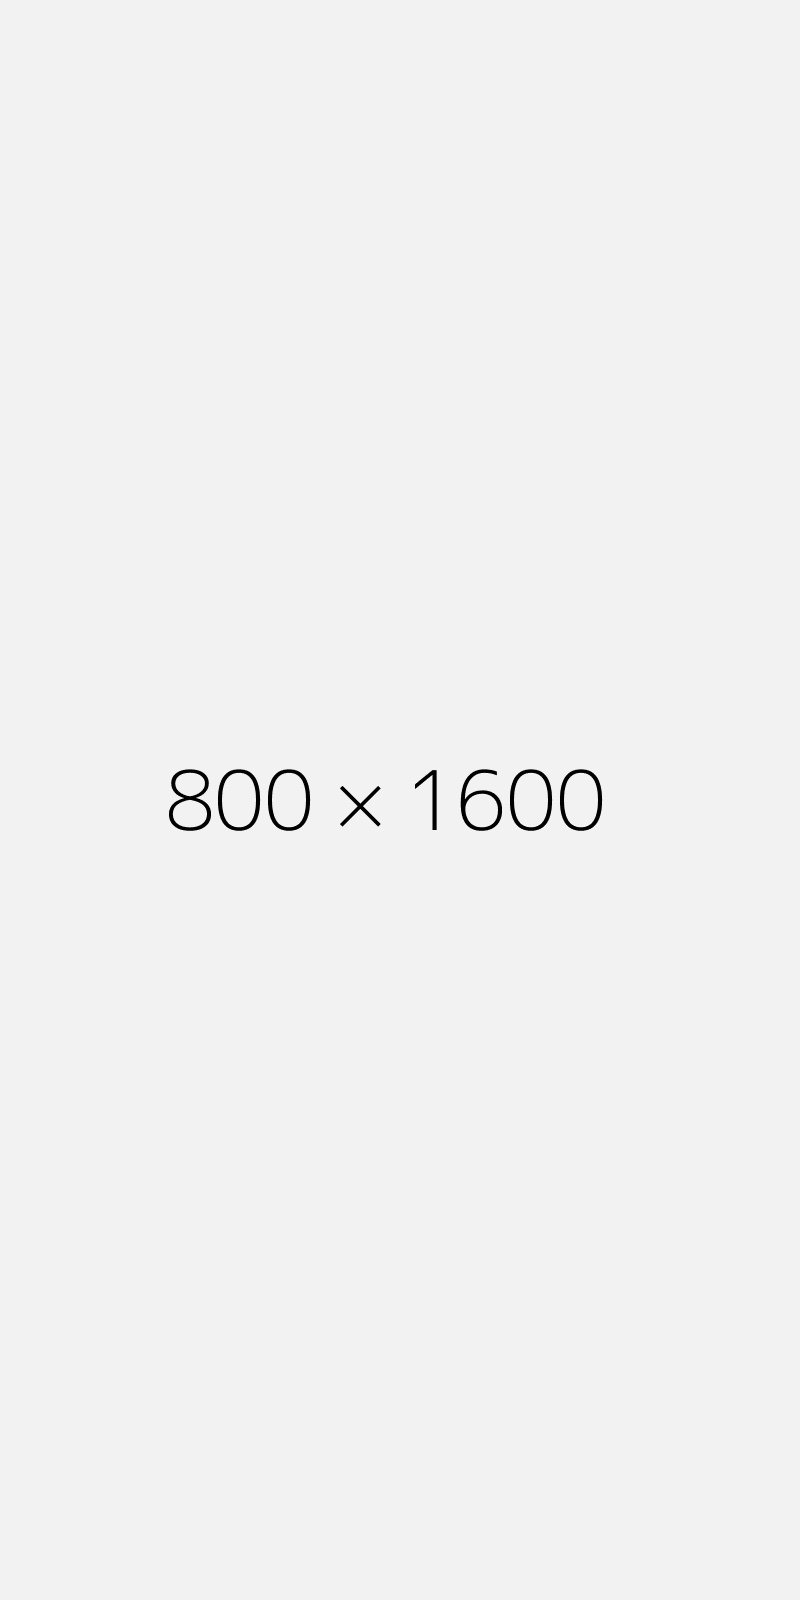
\includegraphics[width=0.5\textwidth]{img/800x1600.png}
\caption{Figure caption.}
\end{figure}

\end{column}
\end{columns}
\end{frame}

%%%%%%%%%%%%%%%%%%%%%%%%%%%%%%%%%%%%%%%%%%%%%%%%%%%%%%%%%%%

\begin{frame}[t]
\frametitle{LAYOUT 6}
\framesubtitle{Text + Two Images, Two Columns}

\begin{columns}[t]
  \begin{column}{0.45\textwidth}
    \lipsum[7]
    \vskip0.5cm%
    \lipsum[8]
  \end{column}

  \begin{column}{0.45\textwidth}
    \begin{figure}[t]
      
\includegraphics[width=0.4\textwidth]{img/1600x1600.png}
      \caption{The other figure caption.}
    \end{figure}
    \begin{figure}[t]
      
\includegraphics[width=0.4\textwidth]{img/1600x1600.png}
      \caption{Yet another figure caption.}
    \end{figure}
\end{column}

\end{columns}
\end{frame}

%%%%%%%%%%%%%%%%%%%%%%%%%%%%%%%%%%%%%%%%%%%%%%%%%%%%%%%%%%%

\begin{frame}[t]
\frametitle{LAYOUT 7}
\framesubtitle{Text + Wide image, Two Columns}

\begin{columns}[t]
\begin{column}{0.45\textwidth}
\lipsum[8][1-4]
\end{column}

\begin{column}{0.45\textwidth}
\lipsum[9][1-4]
\end{column}
\end{columns}
\vskip1.5cm%
\begin{figure}[t]
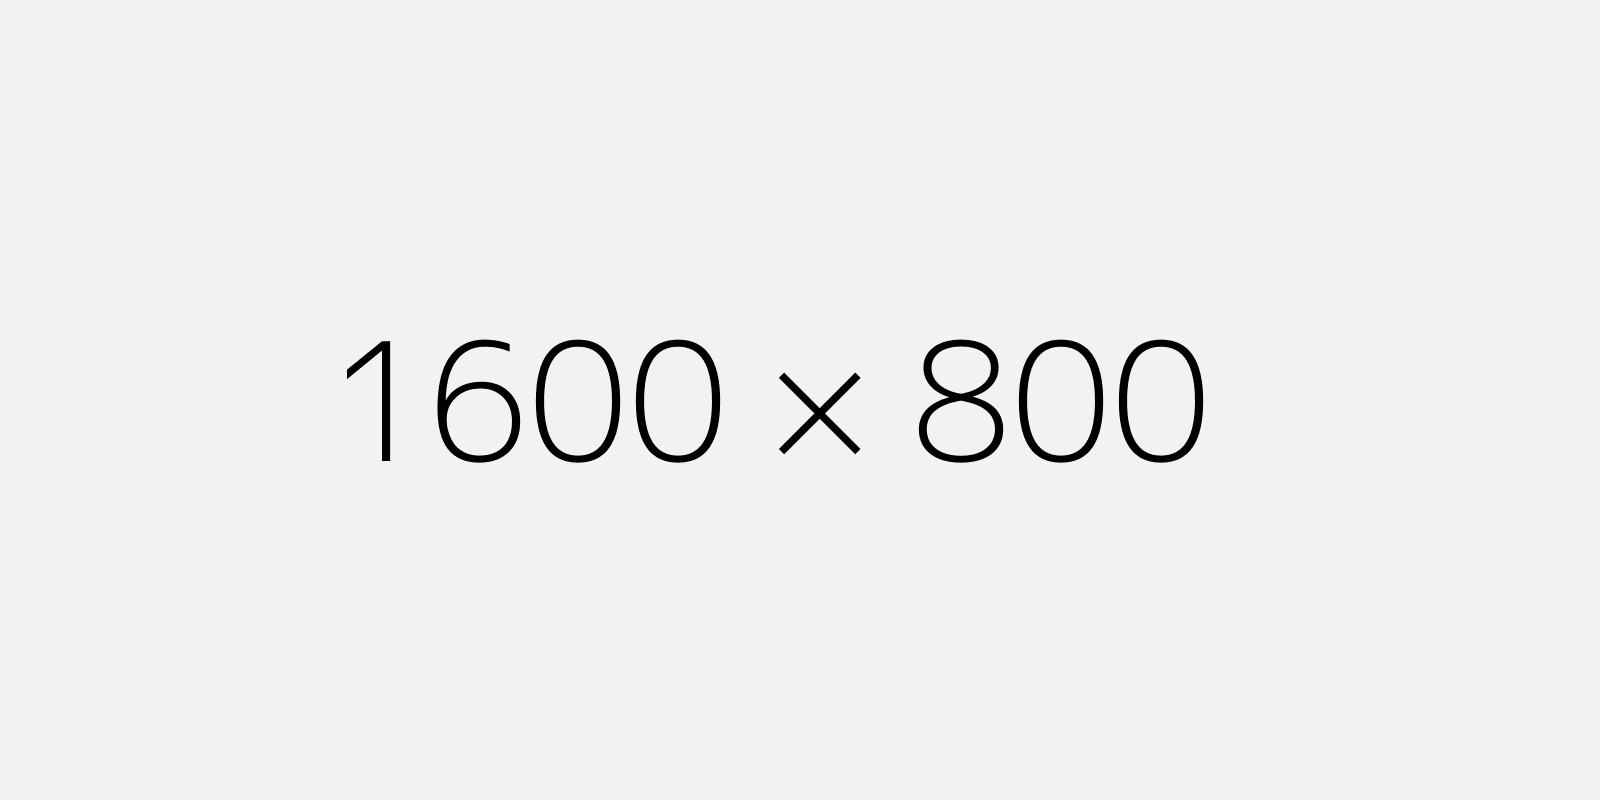
\includegraphics[width=0.6\textwidth]{img/1600x800.png}
\caption{An alternate classification of the decision making process.}
\end{figure}

\end{frame}

%%%%%%%%%%%%%%%%%%%%%%%%%%%%%%%%%%%%%%%%%%%%%%%%%%%%%%%%%%%

\begin{frame}[t]
\frametitle{LAYOUT 8}
\framesubtitle{Two images, Two Columns}

\begin{columns}[t]
  \begin{column}{0.45\textwidth}
    \begin{figure}[t]
      
\includegraphics[width=1\textwidth]{img/1600x1600.png}
      \caption{The other figure caption.}
    \end{figure}
  \end{column}

  \begin{column}{0.45\textwidth}
    \begin{figure}[t]
      
\includegraphics[width=1\textwidth]{img/1600x1600.png}
      \caption{Yet another figure caption.}
    \end{figure}
  \end{column}

\end{columns}

\end{frame}

%%%%%%%%%%%%%%%%%%%%%%%%%%%%%%%%%%%%%%%%%%%%%%%%%%%%%%%%%%%

\begin{frame}[t]
\frametitle{LAYOUT 9}
\framesubtitle{Text + Table, Two Columns}

\begin{columns}[t]
  \begin{column}{0.45\textwidth}
    \lipsum[7]
    \vskip0.5cm%
    \lipsum[8]
  \end{column}

  \begin{column}{0.45\textwidth}
    \begin{table}
      \caption{Table caption.}
      \begin{tabular}{p{0.30\textwidth}p{0.30\textwidth}p{0.30\textwidth}}
        \hline
        \emph{Heading} & \emph{The other heading} & \emph{Yet another heading} \\
        \hline
        Item & \$50 per item & 7 kg \\
        Item & \$20 per item & 3 kg\\
        Item & \$6 per kg & 1.5 kg\\
        Item & \$50 per item & 7 kg \\
        Item & \$20 per item & 3 kg\\
        Item & \$6 per kg & 1.5 kg\\
        \hline
      \end{tabular}
    \end{table}
\end{column}

\end{columns}
\end{frame}

%%%%%%%%%%%%%%%%%%%%%%%%%%%%%%%%%%%%%%%%%%%%%%%%%%%%%%%%%%%

\begin{frame}[t]
\frametitle{LAYOUT 10}
\framesubtitle{Text + List, Two Columns}

\begin{columns}[t]
  \begin{column}{0.45\textwidth}
    \lipsum[7]
    \vskip0.5cm%
    \lipsum[8]
  \end{column}

\begin{column}{0.45\textwidth}
  \emph{Numbered list}

  \begin{enumerate}
    \item First
    \item Second
    \item Third
    \item Fourth
    \item Fifth
  \end{enumerate}

  \vskip0.5cm%

  \emph{Bullet list}

  \begin{itemize}
    \item First
    \item Second
    \item Third
    \item Fourth
    \item Fifth
  \end{itemize}

  \vskip0.5cm%

  \emph{Description}

  \begin{description}
    \item [$\leq$] less than or equal to
    \item [$\geq$] greater than or equal to
    \item [$=$] equal to
  \end{description}

\end{column}

\end{columns}
\end{frame}

%%%%%%%%%%%%%%%%%%%%%%%%%%%%%%%%%%%%%%%%%%%%%%%%%%%%%%%%%%%

%\begin{frame}[t]
%\frametitle{INDEPENDENCE}
%\framesubtitle{Freedom}
%
%\begin{columns}[t]
%\begin{column}{0.45\textwidth}
%\vskip0.5cm%
%\end{column}
%
%\begin{column}{0.45\textwidth}
%\vskip0.5cm%
%\end{column}
%\end{columns}
%\end{frame}

%%%%%%%%%%%%%%%%%%%%%%%%%%%%%%%%%%%%%%%%%%%%%%%%%%%%%%%%%%%

\end{document}